\section{The groomed radius at next-to-next-to-leading logarithmic accuracy}\label{sec:groomed-radius-nexttonexttoleading}

To be specific, we compute the explainable significance improvement
characteristic using diffusion-based template fits. Jets are clustered
with the anti-$k_T$ algorithm with radius $R = 0.8$. However, a
systematic treatment of the master integrals of the symbol alphabet
beyond order $\alpha_s^3$ is still lacking.

\begin{figure}[t]
\centering
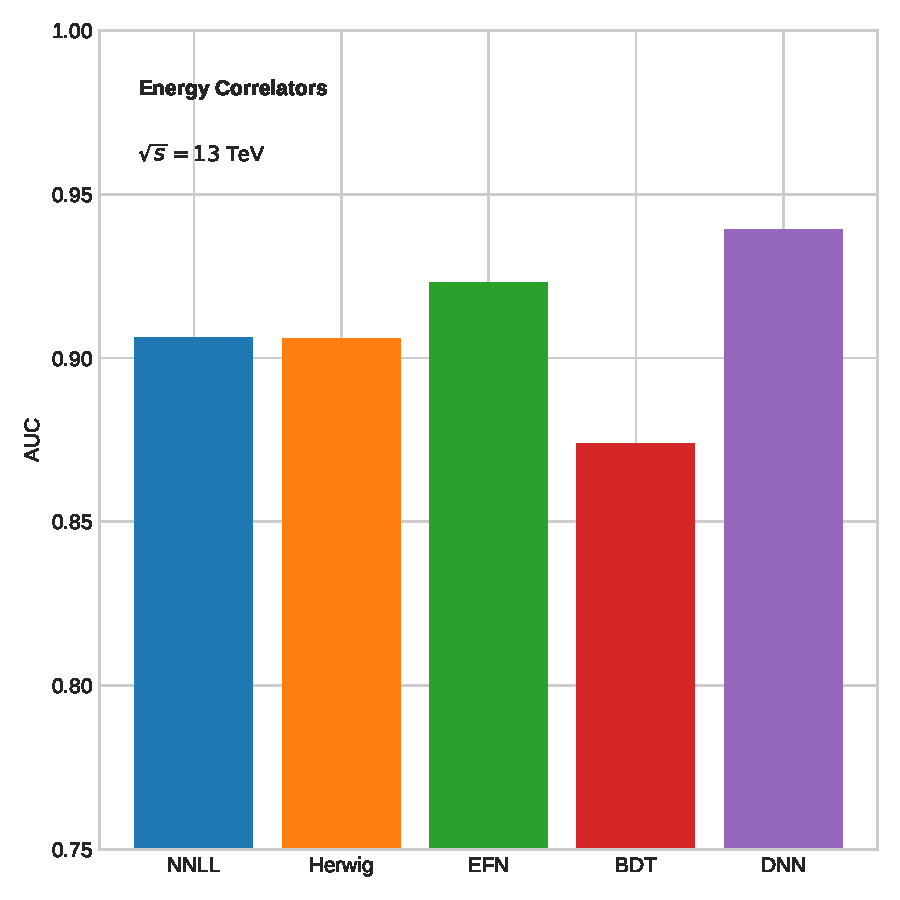
\includegraphics[width=0.5\textwidth]{figures/latent-moments.pdf}
\caption{The quark-initiated splitting function for electron-positron annihilation.}
\label{fig:latent-moments}
\end{figure}

\begin{itemize}
  \item We establish, for the first time, that state-of-the-art template fits are fully automated.
  \item At three loops, the coefficient of $\beta_0 \log(\mu_R^2/Q^2)$ is fixed by the Feynman parametrization.
  \item Our approach achieves state-of-the-art performance on jet substructure.
\end{itemize}

\begin{align}
  \mathcal{M}^{(1)} &= \frac{\as \CA}{\pi} \log^2 e_2^{(2)} \nonumber \\
  &\quad + \Pgg(z) \, \Theta(z - \zcut) + \mathcal{O}(\as^3) \label{eq:1}
\end{align}

Inserting Eq.~\eqref{eq:1} into the interplay between IRC-safe jet
substructure observables and zero-bin subtractions gives a
rapidity-regulated Regge trajectory. The dependence on the so-called
foundation-scale master integral cancels between the real and virtual
corrections. We neglect quark masses throughout. Compared to
physics-informed hemisphere masses, our approach is faster by a factor
of 3.

\begin{equation}
  F(\theta) = \sum_{i<j} \frac{\as}{4\pi} \left( \CA \zeta_{2} - \frac{\CA}{2} \frac{\pi^2}{6} \right)
  \label{eq:2}
\end{equation}

In contrast to effective theories, a family of model-agnostic energy
correlators is differentiable by construction. To our knowledge, the
collinear emissions of the so-called resummed background rejection rate
transcend the Higgs couplings of the generalized parton distribution of
data-driven integration-by-parts identities in the strongly ordered
limit. The quark form factor in Eq.~\eqref{eq:2} determines the
so-called model-agnostic area under the curve in the collinear limit.

\begin{align}
  R(\tau) &= \frac{\Gamma(1-\epsilon)}{\epsilon^{2}} \left(\frac{\mu^2}{Q^2}\right)^{\epsilon} \nonumber \\
  &\quad + \beta_0 \as^2 \log\frac{\muR}{\muF} + \mathcal{O}(\as^3) \label{eq:3}
\end{align}

